
\documentclass[letterpaper,hide notes,xcolor={table,svgnames},pdftex,10pt]{beamer}
\def\showexamples{t}


%\usepackage[svgnames]{xcolor}

%% Demo talk
%\documentclass[letterpaper,notes=show]{beamer}

\usecolortheme{crane}
\setbeamertemplate{navigation symbols}{}

\usetheme{MyPittsburgh}
%\usetheme{Frankfurt}

%\usepackage{tipa}

\usepackage{hyperref}
\usepackage{graphicx,xspace}
\usepackage[normalem]{ulem}

\newcommand\SF[1]{$\bigstar$\footnote{SF: #1}}

\usepackage[default]{sourcesanspro}
\usepackage[T1]{fontenc}

\newcounter{tmpnumSlide}
\newcounter{tmpnumNote}

% old question code
%\newcommand\question[1]{{$\bigstar$ \small \onlySlide{2}{#1}}}
% \newcommand\nquestion[1]{\ifdefined \presentationonly \textcircled{?} \fi \note{\par{\Large \textbf{?}} #1}}
% \newcommand\nanswer[1]{\note{\par{\Large \textbf{A}} #1}}


 \newcommand\mnote[1]{%
   \addtocounter{tmpnumSlide}{1}
   \ifdefined\showcues {~\tiny\fbox{\arabic{tmpnumSlide}}}\fi
   \note{\setlength{\parskip}{1ex}\addtocounter{tmpnumNote}{1}\textbf{\Large \arabic{tmpnumNote}:} {#1\par}}}

\newcommand\mmnote[1]{\note{\setlength{\parskip}{1ex}#1\par}}

%\newcommand\mnote[2][]{\ifdefined\handoutwithnotes {~\tiny\fbox{#1}}\fi
% \note{\setlength{\parskip}{1ex}\textbf{\Large #1:} #2\par}}

%\newcommand\mnote[2][]{{\tiny\fbox{#1}} \note{\setlength{\parskip}{1ex}\textbf{\Large #1:} #2\par}}

\newcommand\mquestion[2]{{~\color{red}\fbox{?}}\note{\setlength{\parskip}{1ex}\par{\Large \textbf{?}} #1} \note{\setlength{\parskip}{1ex}\par{\Large \textbf{A}} #2\par}\ifdefined \presentationonly \pause \fi}

\newcommand\blackboard[1]{%
\ifdefined   \showblackboard
  {#1}
  \else {\begin{center} \fbox{\colorbox{blue!30}{%
         \begin{minipage}{.95\linewidth}%
           \hspace{\stretch{1}} Some space intentionally left blank; done at the blackboard.%
         \end{minipage}}}\end{center}}%
         \fi%
}



%\newcommand\q{\tikz \node[thick,color=black,shape=circle]{?};}
%\newcommand\q{\ifdefined \presentationonly \textcircled{?} \fi}

\usepackage{listings}
\lstset{%
  keywordstyle=\bfseries,
  aboveskip=15pt,
  belowskip=15pt,
  captionpos=b,
  identifierstyle=\ttfamily,
  escapeinside={(*@}{@*)},
  stringstyle=\ttfamiliy,
  frame=lines,
  numbers=left, basicstyle=\scriptsize, numberstyle=\tiny, stepnumber=0, numbersep=2pt}

\usepackage{siunitx}
\newcommand\sius[1]{\num[group-separator = {,}]{#1}\si{\micro\second}}
\newcommand\sims[1]{\num[group-separator = {,}]{#1}\si{\milli\second}}
\newcommand\sins[1]{\num[group-separator = {,}]{#1}\si{\nano\second}}
\sisetup{group-separator = {,}, group-digits = true}

%% -------------------- tikz --------------------
\usepackage{tikz}
\usetikzlibrary{positioning}
\usetikzlibrary{arrows,backgrounds,automata,decorations.shapes,decorations.pathmorphing,decorations.markings,decorations.text}

\tikzstyle{place}=[circle,draw=blue!50,fill=blue!20,thick, inner sep=0pt,minimum size=6mm]
\tikzstyle{transition}=[rectangle,draw=black!50,fill=black!20,thick, inner sep=0pt,minimum size=4mm]

\tikzstyle{block}=[rectangle,draw=black, thick, inner sep=5pt]
\tikzstyle{bullet}=[circle,draw=black, fill=black, thin, inner sep=2pt]

\tikzstyle{pre}=[<-,shorten <=1pt,>=stealth',semithick]
\tikzstyle{post}=[->,shorten >=1pt,>=stealth',semithick]
\tikzstyle{bi}=[<->,shorten >=1pt,shorten <=1pt, >=stealth',semithick]

\tikzstyle{mut}=[-,>=stealth',semithick]

\tikzstyle{treereset}=[dashed,->, shorten >=1pt,>=stealth',thin]

\usepackage{ifmtarg}
\usepackage{xifthen}
\makeatletter
% new counter to now which frame it is within the sequence
\newcounter{multiframecounter}
% initialize buffer for previously used frame title
\gdef\lastframetitle{\textit{undefined}}
% new environment for a multi-frame
\newenvironment{multiframe}[1][]{%
\ifthenelse{\isempty{#1}}{%
% if no frame title was set via optional parameter,
% only increase sequence counter by 1
\addtocounter{multiframecounter}{1}%
}{%
% new frame title has been provided, thus
% reset sequence counter to 1 and buffer frame title for later use
\setcounter{multiframecounter}{1}%
\gdef\lastframetitle{#1}%
}%
% start conventional frame environment and
% automatically set frame title followed by sequence counter
\begin{frame}%
\frametitle{\lastframetitle~{\normalfont(\arabic{multiframecounter})}}%
}{%
\end{frame}%
}
\makeatother

\makeatletter
\newdimen\tu@tmpa%
\newdimen\ydiffl%
\newdimen\xdiffl%
\newcommand\ydiff[2]{%
    \coordinate (tmpnamea) at (#1);%
    \coordinate (tmpnameb) at (#2);%
    \pgfextracty{\tu@tmpa}{\pgfpointanchor{tmpnamea}{center}}%
    \pgfextracty{\ydiffl}{\pgfpointanchor{tmpnameb}{center}}%
    \advance\ydiffl by -\tu@tmpa%
}
\newcommand\xdiff[2]{%
    \coordinate (tmpnamea) at (#1);%
    \coordinate (tmpnameb) at (#2);%
    \pgfextractx{\tu@tmpa}{\pgfpointanchor{tmpnamea}{center}}%
    \pgfextractx{\xdiffl}{\pgfpointanchor{tmpnameb}{center}}%
    \advance\xdiffl by -\tu@tmpa%
}
\makeatother
\newcommand{\copyrightbox}[3][r]{%
\begin{tikzpicture}%
\node[inner sep=0pt,minimum size=2em](ciimage){#2};
\usefont{OT1}{phv}{n}{n}\fontsize{4}{4}\selectfont
\ydiff{ciimage.south}{ciimage.north}
\xdiff{ciimage.west}{ciimage.east}
\ifthenelse{\equal{#1}{r}}{%
\node[inner sep=0pt,right=1ex of ciimage.south east,anchor=north west,rotate=90]%
{\raggedleft\color{black!50}\parbox{\the\ydiffl}{\raggedright{}#3}};%
}{%
\ifthenelse{\equal{#1}{l}}{%
\node[inner sep=0pt,right=1ex of ciimage.south west,anchor=south west,rotate=90]%
{\raggedleft\color{black!50}\parbox{\the\ydiffl}{\raggedright{}#3}};%
}{%
\node[inner sep=0pt,below=1ex of ciimage.south west,anchor=north west]%
{\raggedleft\color{black!50}\parbox{\the\xdiffl}{\raggedright{}#3}};%
}
}
\end{tikzpicture}
}


%% --------------------

%\usepackage[excludeor]{everyhook}
%\PushPreHook{par}{\setbox0=\lastbox\llap{MUH}}\box0}

%\vspace*{\stretch{1}

%\setbox0=\lastbox \llap{\textbullet\enskip}\box0}

\setlength{\parskip}{\fill}

\newcommand\noskips{\setlength{\parskip}{1ex}}
\newcommand\doskips{\setlength{\parskip}{\fill}}

\newcommand\xx{\par\vspace*{\stretch{1}}\par}
\newcommand\xxs{\par\vspace*{2ex}\par}
\newcommand\tuple[1]{\langle #1 \rangle}
\newcommand\code[1]{{\sf \footnotesize #1}}
\newcommand\ex[1]{\uline{Example:} \ifdefined \presentationonly \pause \fi
  \ifdefined\showexamples#1\xspace\else{\uline{\hspace*{2cm}}}\fi}

\newcommand\ceil[1]{\lceil #1 \rceil}


\AtBeginSection[]
{
   \begin{frame}
       \frametitle{Outline}
       \tableofcontents[currentsection]
   \end{frame}
}



\pgfdeclarelayer{edgelayer}
\pgfdeclarelayer{nodelayer}
\pgfsetlayers{edgelayer,nodelayer,main}

\tikzstyle{none}=[inner sep=0pt]
\tikzstyle{rn}=[circle,fill=Red,draw=Black,line width=0.8 pt]
\tikzstyle{gn}=[circle,fill=Lime,draw=Black,line width=0.8 pt]
\tikzstyle{yn}=[circle,fill=Yellow,draw=Black,line width=0.8 pt]
\tikzstyle{empty}=[circle,fill=White,draw=Black]
\tikzstyle{bw} = [rectangle, draw, fill=blue!20, 
    text width=4em, text centered, rounded corners, minimum height=2em]
    
    \newcommand{\CcNote}[1]{% longname
	This work is licensed under the \textit{Creative Commons #1 3.0 License}.%
}
\newcommand{\CcImageBy}[1]{%
	\includegraphics[scale=#1]{creative_commons/cc_by_30.pdf}%
}
\newcommand{\CcImageSa}[1]{%
	\includegraphics[scale=#1]{creative_commons/cc_sa_30.pdf}%
}
\newcommand{\CcImageNc}[1]{%
	\includegraphics[scale=#1]{creative_commons/cc_nc_30.pdf}%
}
\newcommand{\CcGroupBySa}[2]{% zoom, gap
	\CcImageBy{#1}\hspace*{#2}\CcImageNc{#1}\hspace*{#2}\CcImageSa{#1}%
}
\newcommand{\CcLongnameByNcSa}{Attribution-NonCommercial-ShareAlike}

\newenvironment{changemargin}[1]{% 
  \begin{list}{}{% 
    \setlength{\topsep}{0pt}% 
    \setlength{\leftmargin}{#1}% 
    \setlength{\rightmargin}{1em}
    \setlength{\listparindent}{\parindent}% 
    \setlength{\itemindent}{\parindent}% 
    \setlength{\parsep}{\parskip}% 
  }% 
  \item[]}{\end{list}} 




\title{Lecture 10 --- Symmetric Multiprocessing }

\author{Jeff Zarnett \\ \small \texttt{jzarnett@uwaterloo.ca}}
\institute{Department of Electrical and Computer Engineering \\
  University of Waterloo}
\date{\today}


\begin{document}

\begin{frame}
  \titlepage

 \end{frame}

 
\begin{frame}
\frametitle{Multiprocessing}

Not that long ago, a typical computer had one processor with one core. 

It could accordingly do exactly one thing at a time. 

1 processor: 1 general purpose processor that executes user processes. 

There may be special-purpose processors in the system (RAID controller). 

Only one general purpose processor so we call it a uniprocessor system.



\end{frame}

 
\begin{frame}
\frametitle{Multiprocessing}

Now, desktops, laptops, and even cell phones are using multi-core processors.

A quad-core processor may be executing four different instructions from four different threads at the same time. 

In theory, multiple processors may mean that we can get more work done in the same amount of (wall clock) time, but this is not a guarantee. 

Plus, if one of the CPUs in a two-CPU system fails, the system can likely carry on at a reduced performance level.

\end{frame}

 
\begin{frame}
\frametitle{(A)symmetric Multiprocessing}

Multiprocessor systems can be \alert{asymmetric} or \alert{symmetric}.

Asymmetric: there is a \alert{boss} processor and \alert{workers}.

Symmetric: the workers are in charge and all processors are equal, comrade!

We are mostly familiar with symmetric systems.

\end{frame}

 
\begin{frame}
\frametitle{Symmetric Multiprocessing}


A formal definition of SMP:

\begin{enumerate}
	\item There are two or more general purpose processors.
	\item The processors share the same main memory and I/O devices and are interconnected by a bus.
	\item All processors are capable of performing the same functions.
	\item The system is controlled by an OS that provides interaction between processors and their programs.
\end{enumerate}

\end{frame}

 
\begin{frame}
\frametitle{SMP Organization}

\begin{center}
	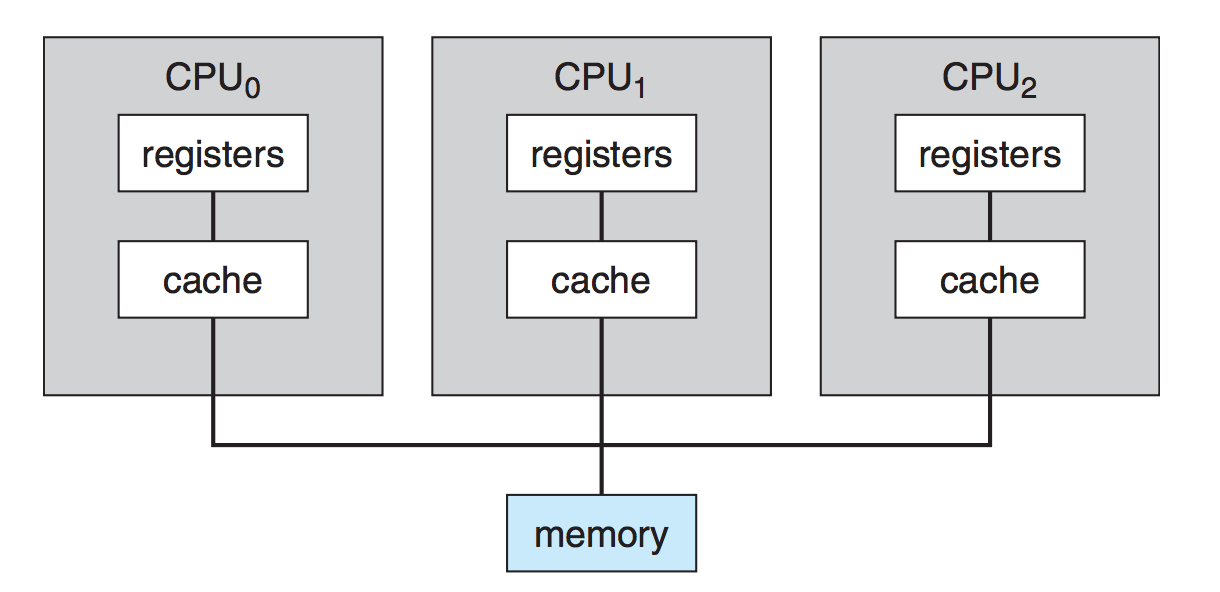
\includegraphics[width=0.75\textwidth]{images/smp-architecture.png}
\end{center}


\end{frame}

 
\begin{frame}
\frametitle{Terminology Note}


Terminology note: we often refer to a logical processing unit as a \alert{core}. 

CPU may refer to a physical chip that contains 1+ logical processing units. 

As far as the operating system is concerned, it does not much matter if a system has four cores in four physical chips or four cores in one chip.

Either way, there are four units that can execute instructions.



\end{frame}

 
\begin{frame}
\frametitle{Execution}

1 process, 1 thread: it does not matter how many cores are available.\\
\quad At most one core will be used to execute this task. 

If there are multiple processes, each process can execute on a different core. 

But what if there are more processes and threads than available cores?

We can hope that the processes get blocked frequently enough and long enough?



\end{frame}

 
\begin{frame}
\frametitle{Execution}

Switch between the different tasks via a procedure we call \alert{time slicing}. 

So thread 1 would execute for a designated period, such as 20 ms, then thread 2 for 20 ms, then thread 3 for 20 ms, then back to thread 1 for 20 ms. 

To the user, it seems like threads 1, 2, and 3 are being executed in parallel.\\
\quad 20 ms is fast enough that the user does not notice the difference.

\end{frame}

 
\begin{frame}
\frametitle{Single Core Execution}

\begin{center}
	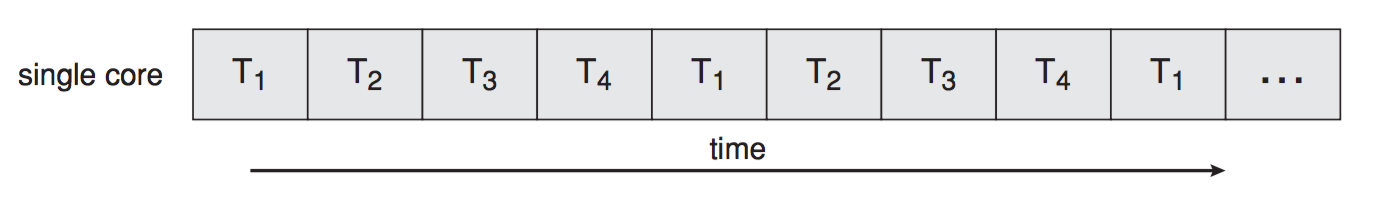
\includegraphics[width=\textwidth]{images/single-core-execution.png}
\end{center}

\end{frame}

 
\begin{frame}
\frametitle{Multi Core Execution}

Time slicing will still occur, if necessary:

\begin{center}
	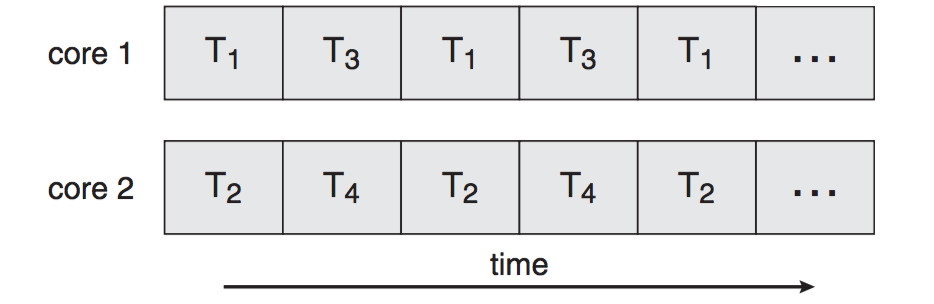
\includegraphics[width=\textwidth]{images/dual-core-execution.png}
\end{center}


\end{frame}

 

\begin{frame}
\frametitle{Parallelism}

Multiple threads at the same time = tasks completed faster?

\end{frame}

\begin{frame}
\frametitle{Parallelism and Speedup}

Depends on the nature of the task!

Fully parallelized: 2 $\times$ Threads = 2 $\times$ Speed

Partially parallelized: 2 $\times$ Threads = $(1 < n < 2)$ $\times$ Speed

Cannot be parallelized: 2 $\times$ Threads = $1$ $\times$ Speed

\end{frame}

 
\begin{frame}
\frametitle{Speedup Example}


Suppose: a task that can be executed in 5~s, containing a parallelizable loop.

Initialization and recombination code in this routine requires 400~ms. 

So with one processor executing, it would take about 4.6~s to execute the loop. 

Split it up and execute on two processors: about 2.3~s to execute the loop. 

Add to that the setup and cleanup time of 0.4~s and we get a total time of 2.7~s. 

Completing the task in 2.7~s rather than 5~s represents a speedup of about~46\%.

\end{frame}

 
\begin{frame}
\frametitle{Amdahl's Law}

Gene Amdahl came up with a formula for the general case of how much faster a task can be completed based on how many processors we have available. 

Let us define $S$ as the portion of the application that must be performed serially and $N$ as the number of processing cores available. 

Amdahl's Law:

\begin{center}
speedup $\leq$ {\huge $\frac{1}{S + \frac{1-S}{N}}$}
\end{center}

\end{frame}

 
\begin{frame}
\frametitle{Amdahl's Law}

Take the limit as $N \rightarrow$ infinity and you will find the speedup converges to $\frac{1}{S}$.


The limiting factor on how much additional processors help is the size of $S$.

Matches our intuition of how it should work.

\end{frame}

 
\begin{frame}
\frametitle{Amdahl's Law on the 5~s Task}

Applying this formula to the example from earlier:

\begin{center}
	\begin{tabular}{l|l}
	\textbf{Processors} & \textbf{Run Time (s)} \\ \hline
	1 & 5\\
	2 & 2.7\\
	4 & 1.55\\
	8 & 0.975\\
	16 & 0.6875 \\
	32 & 0.54375 \\
	64 & 0.471875 \\
	128 & 0.4359375\\
	\end{tabular}
\end{center}

\end{frame}

 
\begin{frame}
\frametitle{Observations on the 5~s Task}

1. Diminishing returns as we add more processors.

2. Converges on 0.4~s.

The most we could speed up this code is by a factor of $\frac{5}{0.4}\approx 12.5$.

But that would require infinite processors (and therefore infinite money).

\end{frame}

 
\begin{frame}
\frametitle{Merge Sort Example}

Recall from data structures and algorithms the concept of merge sort. 

This is a divide-and-conquer algorithm like binary search. 

Split the array of values up into smaller pieces, sort those, and then merge the smaller pieces together to have sorted data.


\end{frame}

 
\begin{frame}
\frametitle{Merge Sort Example}

\begin{center}
	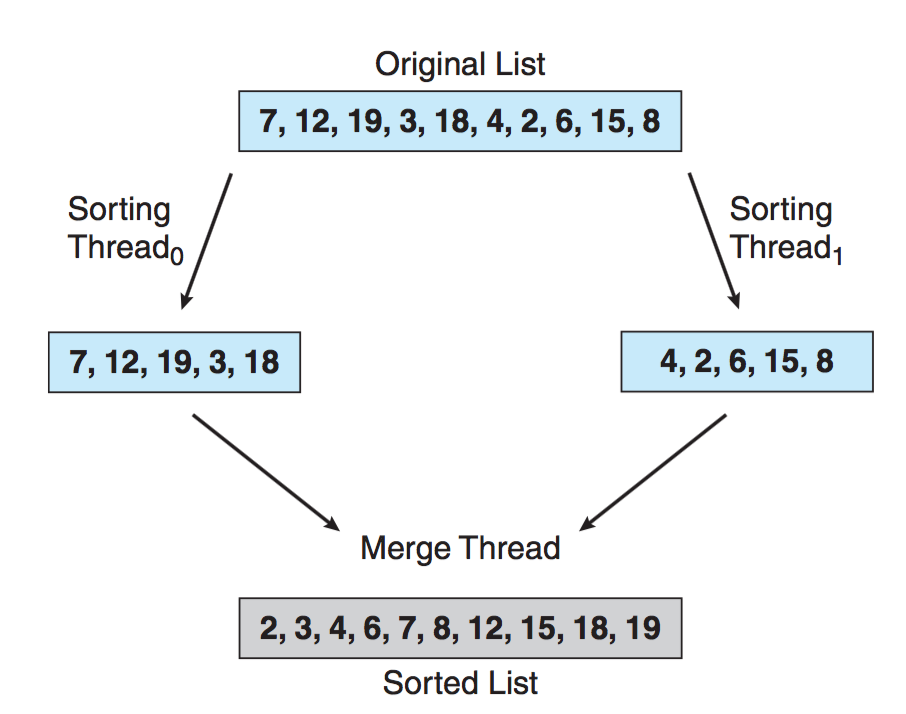
\includegraphics[width=0.75\textwidth]{images/multithread-sort.png}
\end{center}


\end{frame}
 
\begin{frame}
\frametitle{Merge Sort}

For a small array it makes sense to use one of the simple algorithms like insertion sort.\\
\quad  (despite $\Theta(n^{2})$ worst-case runtime). 

You may have seen something similar in optimized binary search algorithms where, at some point, a linear search is used. 

So let us begin with the code for the insertion sort routine:

\end{frame}
 
\begin{frame}[fragile]
\frametitle{Insertion Sort Code}

\begin{verbatim}
void insertion_sort( double *array, size_t a, size_t b ) {
  size_t j, k;
  double tmp;
  for ( int k = a + 1; k < b; ++k ) { 
    tmp = array[k];
    
    for ( int j = k; j > a; --j ) {
      if ( array[j - 1] > tmp ) {
        array[j] = array[j - 1];
      } else {
        array[j] = tmp;
        break;
      }
    }
    if ( tmp < array[a] ) {
      array[a] = tmp;
    }
  } 
}
\end{verbatim}

\end{frame}
 
\begin{frame}
\frametitle{The Merge Sort}


If the list is below a certain size, perform the insertion sort. 

Otherwise, divide the list in half and call merge sort recursively on each half.

Merge the results of those two lists.

\end{frame}
 
\begin{frame}[fragile]
\frametitle{Merge Code}

{\tiny
\begin{verbatim}
#include <assert.h>

// Merge the entries from a to b - 1 and from b to c - 1 
void merge( double *array, size_t a, size_t b, size_t c ) {
  assert( a <= b && b <= c );
  
  size_t i = 0, j = a, k = b;
  double *sorted_array = (double *) malloc( (c - a)*sizeof( double ) );
  
  while ( j < b && k < c ) {
    if ( array[j] <= array[k] ) {
      sorted_array[i] = array[j];
      ++j; 
    } else {
      sorted_array[i] = array[k];
      ++k; 
    }
    
    ++i; 
    }
    
  for ( ; j < b; ++i, ++j ) {
    sorted_array[i] = array[j];
  }
    
  for ( ; k < c; ++i, ++k ) {
    sorted_array[i] = array[k];
  }
    
  for ( i = 0, k = a; k < c; ++i, ++k ) {
    array[k] = sorted_array[i];
  }
    
  free( sorted_array );
}
\end{verbatim}
}


\end{frame}
 
\begin{frame}[fragile]
\frametitle{Insertion Sort Code}


\begin{verbatim}
#define USE_INSERTION_SORT 30

void merge_sort( double *array, size_t a, size_t c ) {
  assert( a <= c );
  
  if ( c - a < USE_INSERTION_SORT ) {
    insertion_sort( array, a, c );
    return;
  }
  size_t b = a + (c - a)/2;
  
  merge_sort( array, a, b );
  merge_sort( array, b, c );
  merge( array, a, b, c );
}
\end{verbatim}

\end{frame}

\begin{frame}[fragile]
\frametitle{Argument Structure}


To run this as a new thread, we can pass in only one argument for the parameters to the sort function. 

So we need a \texttt{struct} object to contain the arguments:

\begin{verbatim}
typedef struct interval {
  double *array;
  size_t a;
  size_t c;
} interval_t;
\end{verbatim}


\end{frame}

\begin{frame}[fragile]
\frametitle{User API}

The user does not know that we are going to use a parallel algorithm so the function call should seem somewhat more ``natural'' and delegate to our internal function: 

\begin{verbatim}
void merge_sort( double *array, size_t n ) {
  interval_t arg;
  arg.array = array;
  arg.a = 0;
  arg.c = n;
  merge_sort_internal( &arg );
}
\end{verbatim}

\end{frame}

\begin{frame}[fragile]
\frametitle{Internal Implementation}

{\scriptsize
\begin{verbatim}
void *merge_sort_interal( void *void_arg ) {
  // the argument is an arbitrary pointer
  //   cast it to a pointer to an instance of 'interval_t'
  interval_t *arg = (interval_t *)void_arg;
  if ( ( arg->c - arg->a ) < USE_INSERTION_SORT ) {
    insertion_sort( arg->array, arg->a, arg->c );
    return NULL;
  }
  
  size_t b = arg->a + (arg->c - arg->a)/2;
  
  interval_t arg1, arg2;
  
  arg1.array = arg->array;
  arg1.a = arg->a;
  arg1.c = b;
  
  arg2.array = arg->array;
  arg2.a = b;
  arg2.c = arg->c;
\end{verbatim}
}
\end{frame}

\begin{frame}[fragile]
\frametitle{Internal Implementation}

{\scriptsize
\begin{verbatim}
  pthread_t other_thread;

  // Create a thread to sort the second half
  pthread_create( &other_thread, NULL, merge_sort_interal, &arg2 ); 
  merge_sort_interal( &arg1 );
  
  // Wait for them to finish
  pthread_join( other_thread, NULL );

  merge( arg->array, arg->a, b, arg->c );

  return NULL;
}
\end{verbatim}
}
\end{frame}

\begin{frame}
\frametitle{Execution, Visually}

Execution on an array of capacity 21 and insertion sort threshold of 5:

\begin{center}
	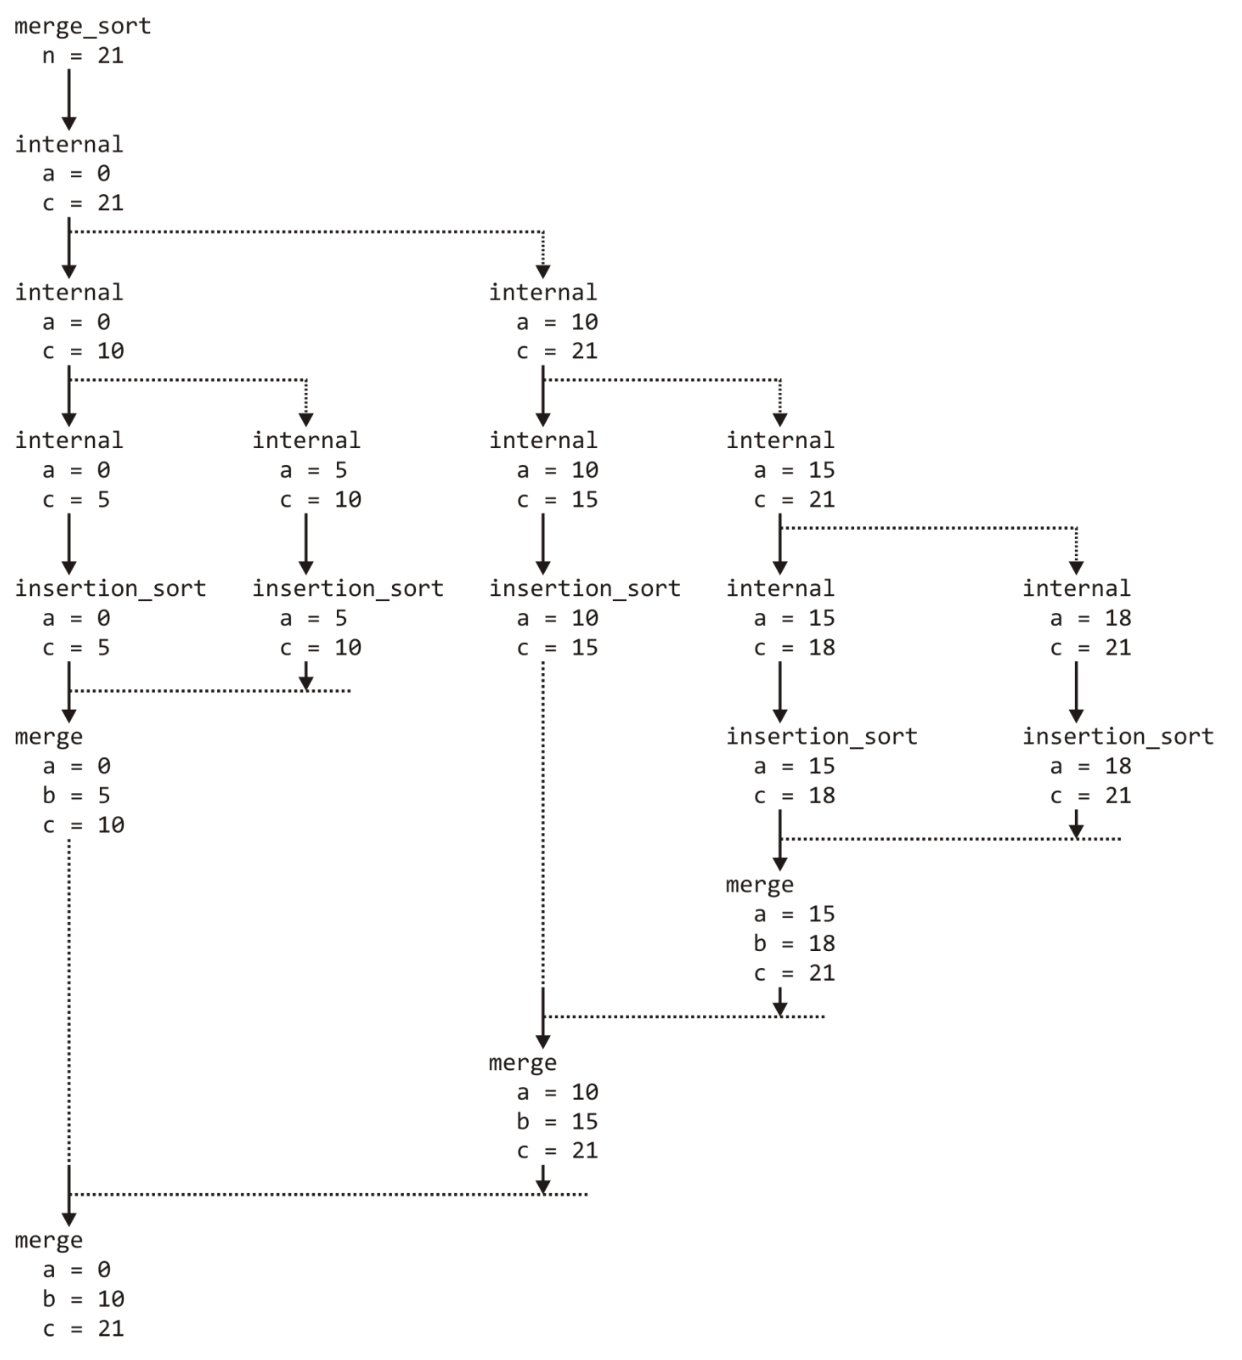
\includegraphics[width=0.6\textwidth]{images/merge-sort-execution.png}
\end{center}
\end{frame}

\begin{frame}
\frametitle{Runtime Analysis}


The runtime of merge sort, according to the data structures and algorithms course is $\Theta(n$ ln$(n))$;

If each of the threads execute on their own core, then the run time will be reduced to $\Theta(n)$.

\end{frame}



\end{document}

